\documentclass[12pt]{report} %fuente a 12pt

% MÁRGENES: 2,5 cm sup. e inf.; 3 cm izdo. y dcho.
\usepackage[
a4paper,
vmargin=2.5cm,
hmargin=3cm
]{geometry}

% INTERLINEADO: Estrecho (6 ptos./interlineado 1,15) o Moderado (6 ptos./interlineado 1,5)
\renewcommand{\baselinestretch}{1.15}
\parskip=6pt

% DEFINICIÓN DE COLORES para portada y listados de código
\usepackage[table]{xcolor}
\definecolor{azulUC3M}{RGB}{0,0,102}
\definecolor{gray97}{gray}{.97}
\definecolor{gray75}{gray}{.75}
\definecolor{gray45}{gray}{.45}

% Soporte para GENERAR PDF/A
\usepackage[a-1b]{pdfx}

% ENLACES
\usepackage{hyperref}
\hypersetup{colorlinks=true,
	linkcolor=black, % enlaces a partes del documento (p.e. índice) en color negro
	urlcolor=blue} % enlaces a recursos fuera del documento en azul

\usepackage{pdfpages}
\setlength{\parindent}{0em}

% EXPRESIONES MATEMATICAS
\usepackage{amsmath,amssymb,amsfonts,amsthm}

\usepackage{txfonts} 
\usepackage[T1]{fontenc}
\usepackage[utf8]{inputenc}

\usepackage{tikz}
\usepackage{pgfplots}

\usepackage[spanish, es-tabla]{babel} 
\usepackage[babel, spanish=spanish]{csquotes}
\AtBeginEnvironment{quote}{\small}

% diseño de PIE DE PÁGINA
\usepackage{fancyhdr}
\pagestyle{fancy}
\fancyhf{}
\renewcommand{\headrulewidth}{0pt}
\rfoot{\thepage}
\fancypagestyle{plain}{\pagestyle{fancy}}

% DISEÑO DE LOS TÍTULOS de las partes del trabajo (capítulos y epígrafes o subcapítulos)
\usepackage{titlesec}
\usepackage{titletoc}
\titleformat{\chapter}[block]
{\large\bfseries\filcenter}
{\thechapter.}
{5pt}
{\MakeUppercase}
{}
\titlespacing{\chapter}{0pt}{0pt}{*3}
\titlecontents{chapter}
[0pt]                                               
{}
{\contentsmargin{0pt}\thecontentslabel.\enspace\uppercase}
{\contentsmargin{0pt}\uppercase}                        
{\titlerule*[.7pc]{.}\contentspage}                 

\titleformat{\section}
{\bfseries}
{\thesection.}
{5pt}
{}
\titlecontents{section}
[5pt]                                               
{}
{\contentsmargin{0pt}\thecontentslabel.\enspace}
{\contentsmargin{0pt}}
{\titlerule*[.7pc]{.}\contentspage}

\titleformat{\subsection}
{\normalsize\bfseries}
{\thesubsection.}
{5pt}
{}
\titlecontents{subsection}
[10pt]                                               
{}
{\contentsmargin{0pt}                          
	\thecontentslabel.\enspace}
{\contentsmargin{0pt}}                        
{\titlerule*[.7pc]{.}\contentspage}  


% DISEÑO DE TABLAS.
\usepackage{multirow} % permite combinar celdas 
\usepackage{caption} % para personalizar el título de tablas y figuras
\usepackage{floatrow} % utilizamos este paquete y sus macros \ttabbox y \ffigbox para alinear los nombres de tablas y figuras de acuerdo con el estilo definido. Para su uso ver archivo de ejemplo 
\usepackage{array} % con este paquete podemos definir en la siguiente línea un nuevo tipo de columna para tablas: ancho personalizado y contenido centrado
\newcolumntype{P}[1]{>{\centering\arraybackslash}p{#1}}
\DeclareCaptionFormat{upper}{#1#2\uppercase{#3}\par}

% Diseño de tabla para ingeniería
\captionsetup[table]{
	format=upper,
	name=TABLA,
	justification=centering,
	labelsep=period,
	width=.75\linewidth,
	labelfont=small,
	font=small,
}

% DISEÑO DE FIGURAS.
\usepackage{graphicx}
\graphicspath{{img/}} %ruta a la carpeta de imágenes

% Diseño de figuras para ingeniería
\captionsetup[figure]{
	format=hang,
	name=Fig.,
	singlelinecheck=off,
	labelsep=period,
	labelfont=small,
	font=small		
}

% NOTAS A PIE DE PÁGINA
\usepackage{chngcntr} %para numeración contínua de las notas al pie
\counterwithout{footnote}{chapter}

% LISTADOS DE CÓDIGO
% soporte y estilo para listados de código. Más información en https://es.wikibooks.org/wiki/Manual_de_LaTeX/Listados_de_código/Listados_con_listings
\usepackage{listings}

% definimos un estilo de listings
\lstdefinestyle{estilo}{ frame=Ltb,
	framerule=0pt,
	aboveskip=0.5cm,
	framextopmargin=3pt,
	framexbottommargin=3pt,
	framexleftmargin=0.4cm,
	framesep=0pt,
	rulesep=.4pt,
	backgroundcolor=\color{gray97},
	rulesepcolor=\color{black},
	%
	basicstyle=\ttfamily\footnotesize,
	keywordstyle=\bfseries,
	stringstyle=\ttfamily,
	showstringspaces = false,
	commentstyle=\color{gray45},     
	%
	numbers=left,
	numbersep=15pt,
	numberstyle=\tiny,
	numberfirstline = false,
	breaklines=true,
	xleftmargin=\parindent
}

\captionsetup[lstlisting]{font=small, labelsep=period}
% fijamos el estilo a utilizar 
\lstset{style=estilo}
\renewcommand{\lstlistingname}{\uppercase{Código}}

\pgfplotsset{compat=1.17} 
%-------------
%	DOCUMENTO
%-------------

\begin{document}
\pagenumbering{roman} % Se utilizan cifras romanas en la numeración de las páginas previas al cuerpo del trabajo
	
%----------
%	PORTADA
%----------	
\begin{titlepage}
	\begin{sffamily}
	\color{azulUC3M}
	\begin{center}
		\begin{figure}[H] %incluimos el logotipo de la Universidad
			\makebox[\textwidth][c]{
\includegraphics[width=16cm]{Portada_Logo.png}}
		\end{figure}
		\vspace{2.5cm}
		\begin{Large}
			Grado en Ingeniería Informática\\			
			2020-2021\\
			\vspace{2cm}		
			\textsl{Apuntes}\\
			\bigskip
		\end{Large}
		 	{\Huge Diseño de Sistemas Operativos}\\
		 	\vspace*{0.5cm}
	 		\rule{10.5cm}{0.1mm}\\
			\vspace*{0.9cm}
			{\LARGE Jorge Rodríguez Fraile\footnote{\href{mailto:100405951@alumnos.uc3m.es}{Universidad: 100405951@alumnos.uc3m.es}  |  \href{mailto:jrf1616@gmail.com}{Personal: jrf1616@gmail.com}}}\\ 
			\vspace*{1cm}
	\end{center}
	\vfill
	\color{black}
		
\includegraphics[width=4.2cm]{img/creativecommons.png}\\
		Esta obra se encuentra sujeta a la licencia Creative Commons\\ \textbf{Reconocimiento - No Comercial - Sin Obra Derivada}
	\end{sffamily}
\end{titlepage}

%----------
%	ÍNDICES
%----------	

%--
% Índice general
%-
\tableofcontents
\thispagestyle{fancy}

%--
% Índice de figuras. Si no se incluyen, comenta las líneas siguientes
%-
\listoffigures
\thispagestyle{fancy}

%--
% Índice de tablas. Si no se incluyen, comenta las líneas siguientes
%-
\listoftables
\thispagestyle{fancy}

%----------
%	TRABAJO
%----------	
\clearpage
\pagenumbering{arabic} % numeración con números arábigos para el resto de la publicación	


%----------
%	COMENZAR A ESCRIBIR AQUI
%----------	


\section{Información}

\begin{quote}
Teorías: Javier García Guzmán

Prácticas: Mat Max Montalvo Martínez
\end{quote}

\chapter{Tema 1: Arquitectura de Sistemas
IoT}

\href{https://learning.oreilly.com/library/view/internet-of-things/9781788470599/a7f866bd-4ac8-47f3-a175-0f10d91a5ce2.xhtml}{Definición
de Internet de las Cosas}

\href{https://learning.oreilly.com/library/view/internet-of-things/9781119456742/part04.xhtml\#part}{Aplicaciones
Actuales de Internet de las Cosas}

\href{https://learning.oreilly.com/library/view/build-your-own/9781484244982/html/474034_1_En_2_Chapter.xhtml}{Arquitectura
de Sistemas de Internet de las Cosas}

\textbf{IoT - Internet de las Cosas}: Consiste en conectar a internet
cualquier dispositivo, vehículo, edificios o en general objetos a los
que se les haya dotado de sensores, actuadores y conexión a la red. Lo
que les permite obtener e intercambiar información. Red de objetos
conectados a internet que aporta valor añadidos a los usuarios que
interactúan con ellos.

Consiste en añadir \textbf{inteligencia computacional} a dispositivos
para mejorar las funcionalidades.

Permite que los dispositivos puedan intercambiar información.

Se busca que sean pequeños y tengan un chip que les permita
\textbf{conectarse a la red} y operar en ella. Lo estandarizo IBM.

El \textbf{top 6 áreas} de aplicación de IoT:

\begin{enumerate}
\def\labelenumi{\arabic{enumi}.}

\item
  \textbf{Industrial/Fabricación}: Automatizar, controlar la
  distribución, gestión de instalaciones.
\item
  \textbf{Transporte/Movilidad:} Coches, tráfico en ciudad, vehículos de
  transporte masivo y transporte industrial.
\item
  \textbf{Energía/Gestión eléctrica}: Predecir consumo, personalizar,
  bien estar de los ocupantes, monitorizar el consumo detallado,
  instalaciones con sensores.
\item
  \textbf{Gestión de inventarios/Comercial}: Saber cuánto queda y pedir,
  facilitar compras.
\item
  \textbf{Ciudad}: Recoge muchas áreas; basura, vigilancia, trafico,
  etc.
\item
  \textbf{Salud:} Investigación, la forma de tratar, las emergencias,
  distribución de información médica y dispositivos.
\end{enumerate}

\textbf{Agricultura de precisión}: Según las previsiones ambientales y
meteorológicas, plagas y demás se calcula el mejor momento para sembrar.
Además, cuando ya está plantado, las condiciones del suelo, cuando regar
y abonar las tierras, así como la recolecta.

\newpage

\section{En IoT de vehículos hay distintos
niveles}

\textbf{0}: Sin automatización.

\textbf{1}: Asistencia en la conducción.

\textbf{2}: Control de carril, lateral y longitudinal.

\textbf{3}: Conducción autónoma, pero el conductor en su puesto, para
riesgos.

\textbf{4}: Conducción autónoma, pero el conductor en su puesto,
supervisar.

\textbf{5}: Conducción totalmente autónoma, sin conductor.

\section{Elementos IoT}

\textbf{Colector}: Recogen información, sensores, o se activan,
actuadores, que se intercambian en internet.

\textbf{Transmisor}: Puertas de enlace, pasarelas, pasan los datos a la
red desde los dispositivos.

\textbf{Agregación + Distribución}: Calculo y procesamiento de la
información.

\textbf{Consumidor}: Los usuarios/clientes acceden a los datos.

\section{Evolución}

3 generaciones.

\begin{enumerate}
\def\labelenumi{\arabic{enumi}.}
\item
  \textbf{RFID y sensores}

  Tecnología de detección por radiofrecuencia.

  Las cosas contengan información, las etiquetas (como NFC, se
  estandarizó para indicar que datos contiene) y tener un dispositivo
  que al acercarlo podamos leerla.
\item
  \textbf{Web services e inter-networking} (2004-2012): Interconexión
  completa de las cosas y la red de las cosas.

  IPv4, HTTP, Bluetooth, TCP, UDP, etc.

  Pasan a tener una manera fácil de conectarse los dispositivos entre sí
  o con internet.
\item
  \textbf{Social, Cloud \& ICN:} La era de la computación en la nube y
  la Internet del futuro.

  En esta generación la lógica pasa a estar en la nube, no en el
  dispositivo.

  Gestión de grandes cantidades de información.

  Seguridad, evitar accesos fraudulentos.
\end{enumerate}

\section{Arquitectura de un Sistema IoT}
\begin{description}
	\item[Dispositivos (Devices)] Sensores y actuadores FÍSICOS, que
	normalmente tienen un microprocesador, que mide el medio físico y
	transforma las mediciones a señales digitales. Su función es tomar
	medidas y procesarlas, pero su función no puede ser solo transmitir la
	información.
	
	Actuador, Sensores, LED, LCD, Beacon (la parte dispositivo), Termostato,
	RFID, Trampa para ratones inteligente, Dispositivos embebidos, etc.
	\item[Pasarela (Gateway)] Dispositivo o protocolo con la capacidad de
	comunicar con internet los dispositivos, para transmitir los datos
	tomados. Su única función es transmitir.
	
	Router, Wifi, GSM, Bluetooth, Zigbee, Raspberry a veces, AMQP, CoAP,
	LoRaWAN (sistema de radio), Wimax.
	
	Un móvil está entre Device y Gateway.
	\item[Plataforma IoT (IoT Platform)] Conjunto de servicios
	orquestados para gestionar una gran red de dispositivos interconectados
	y que proporcionan información a aplicaciones u otros tipos de sistemas
	de información. Gestiona y almacena grandes cantidades de datos y las
	redirige. Funciona como middleware.
	
	Es una nube de servidores que dan servicios:
	
	\begin{enumerate}
		\item \textbf{Message broker y Message bus}: Se encarga de conectar los
		dispositivos físicos con los distintos procesos que forman parte de la
		red de IoT. Manda los datos a todos los que estén conectados a su bus,
		suscritos por API Rest.
		\item
		\textbf{Message router}: Está suscrito al message broker, los mensajes
		que recibe los enriquece; dando información semántica, de contexto, de
		estado y los reenvía a aquellos componentes que van a gestionar la
		lógica de las aplicaciones relacionadas con la nube IoT. Otra cosa que
		hace es transformar datos, descomprimir y decodificar datos para
		hacerlos más fáciles de procesar y tratar.
		\item
		\textbf{Rest API}: Interfaz que usan otros programas para obtener los
		servicios o las funcionalidades de un componente. Esta API se
		caracteriza por ser accesible por http e independiente del estado del
		sistema.
		\item
		\textbf{Data Management}: Para almacenar y gestionar los datos tomados
		en la red.
		\item
		\textbf{Rule engine}: Permite monitorear los mensajes recibidos desde
		el router y permite lanzar distintas acciones en distintos elementos.
		Decide que acción tomar.
		
		Ejem: Si se abre la puerta, entonces avisar de intruso.
		\item
		\textbf{Microservicios}: Proporciona funcionalidades muy específicas a
		través de una interfaz API Rest bien definidas mediante un contrato de
		datos. Muchos los coordina el rule engine. Se busca que este muy
		cohesionado y poco acoplado.
		
		Ejem: El que actualiza la estación meteorológica en el móvil, es un
		proceso muy concreto.
		\item
		\textbf{Device manager}: Permite monitorizar algunos elementos de los
		sensores físicos como si está activo, la batería o si está conectado a
		la red.
		\item
		\textbf{App y User management}: Sistema de permisos que identifica y
		gestiona el acceso de usuarios y aplicaciones.
	\end{enumerate}

	\item[Aplicación (Application)] La interfaz que el usuario utiliza
	para controlar el sistema.

\end{description}

\textbf{iBeacon} es un ejemplo de protocolo y \textbf{Beacon} es el
dispositivo. Ambos están relacionados con dispositivos.

\textbf{Small Data}: Que solo proporcione la información de valor
añadido. Es un conjunto de datos con un volumen y un formato que hacen
que los datos sean accesibles, informativos y procesables.

\textbf{Wimax}: Conjunto de tecnologías y protocolos para aumentar el
alcance de las redes inalámbricas (en vez de 30 metros, 40 kilómetros).

\chapter{Tema 2: Sensores y
Actuadores}

\href{https://learning.oreilly.com/library/view/internet-of-things/9781788470599/d39be056-b166-476e-868e-c415e4dfa886.xhtml}{Introducción
a Sensores y Actuadores} 

Hasta la sección `Up to Functional examples
(putting it all together)' incluida.

\section{Sensores}

Conjunto de componentes electrónicos capaces de detectar cambios físicos
en el entorno y enviar información a otros componentes electrónicos,
generalmente un procesador de computadora.

\textbf{Ejemplos}: Sensor de luz (LDR), sensor de ultrasonidos,
giroscopio, fototransistor, Reed switch, \ldots{}

Los sensores se pueden clasificar en tipos según lo que miden: Gases,
velocidad, flujo, fugas, movimiento, electricidad, \ldots{}

Según la señal que produce:

\begin{itemize}

\item
  \textbf{Analógico}: Produce voltaje analógico constante de lo medido.
  El grafico de voltaje sobre el tiempo debe ser continuo y suave.

\begin{figure}[H]
	\ffigbox[\FBwidth]
	{\caption{Diagrama de voltaje Sensor Analogico}}
	{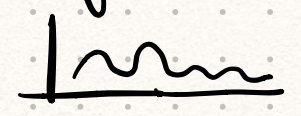
\includegraphics[scale=.5]{image-20210307210139988.png}}
\end{figure}

    Sensor de presión, sensor de luz, sensor de temperatura,
    acelerómetro, sensor de sonido.

\item
  \textbf{Digital}: Produce un voltaje discreto, por lo general tendrá
  uno u otro de dos valores, 0V (apagado) a 5V (encendido). Gracias a la
  miniaturización hay más dado que se puede introducir un conversor.

\begin{figure}[H]
	\ffigbox[\FBwidth]
	{\caption{Diagrama de voltaje Sensor Digital}}
	{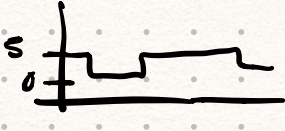
\includegraphics[scale=.5]{image-20210307210421078.png}}
\end{figure}

    Sensor de ultrasonidos, sensor de infrarrojos, acelerómetro, sensor
    de sonido (suele ser analógico), sensor de temperatura.
\end{itemize}

Según si necesitan energía:

\begin{itemize}

\item
  \textbf{Sensor activo}: Siempre \textbf{necesitan} su propia fuente de
  energía.

  \begin{itemize}
  
  \item
    Sensor de ultrasonidos, radar, LiDAR, sensor de humedad, cámara
    infrarroja.
  \end{itemize}
\item
  \textbf{Sensor pasivo}: \textbf{No necesitan} una fuente de energía,
  usan factores externos para alimentarse.

  \begin{itemize}
  
  \item
    Sensor infrarrojo (fotodiodo infrarrojo), sensor PIR, sensor de luz
    (LDR)
  \end{itemize}
\end{itemize}

\textbf{Sensor piezoeléctrico:}

\begin{enumerate}
\def\labelenumi{\arabic{enumi}.}

\item
  Un cristal piezoeléctrico se coloca entre dos placas de metal que
  están en perfecto equilibrio y conduce ninguna corriente eléctrica.
\item
  Las placas de metal aplican tensión o fuerza mecánica sobre el
  material que hace que las cargas eléctricas del cristal se
  desequilibren.
\item
  Las placas de metal recogen esas cargas y producen un voltaje y envía
  una corriente eléctrica a través de un circuito.
\end{enumerate}

\section{Actuadores}

Cualquier dispositivo capaz de intervenir para cambiar las condiciones
físicas del entorno generando los datos.

\textbf{Ejemplos}: Display, LED, servomotor, motor de paso a paso,
Relay, solenoide, actuadores lineales, \ldots{}

\section{Factores de selección de Sensores y
Actuadores}

\textbf{Factores ambientales}: Temperatura, Humedad, Corrosión,
Interferencia electromagnética, Tamaño, Rudeza y Consumo de energía.

\textbf{Factores económicos}: Coste, Disponibilidad y Tiempo de vida.

\textbf{Factores característicos del sensor}: Sensibilidad, Rango,
Estabilidad, Repetibilidad, Rango de error, Tiempo de respuesta y
Linealidad.

\chapter{Tema 3: Sistemas operativos embebidos para Dispositivos
IoT}

\href{https://learning.oreilly.com/library/view/embedded-systems-architecture/9780123821966/xhtml/CHP001.html#CHP001titl}{Introducción a los Sistemas Embebidos} Solo capítulo 1

\href{https://learning.oreilly.com/library/view/embedded-systems-architecture/9780123821966/xhtml/CHP009.html#CHP009titl}{Sistemas
Operativos Embebidos} Capítulo 9

\href{https://learning.oreilly.com/library/view/embedded-systems-architecture/9780123821966/xhtml/CHP008.html#CHP008titl}{Drivers de Dispositivos
} Hasta el encabezado "8.1 Example 1: Device Drivers for Interrupt Handling"

\href{https://learning.oreilly.com/library/view/embedded-systems-architecture/9780123821966/xhtml/CHP010.html#CHP010titl}{Middleware
} Secciones 10.1 y 10.2

\section{¿Que es un sistema embebido o
integrado?}

Sistemas basados en computadora que no parecen ser computadoras, la complejidad esta oculta al usuario.

Son sistemas que integran uno o más sensores y que son capaces de
comunicarse con la red, con capacidades limitadas, por lo que están
entre la capa de Dispositivos y Pasarelas.

Se aplican sobre cosas cotidianas para mejorarla, pero no
proporciona una mayor complejidad del sistema, permite realizar la
mismas funciones o alguna más pero mejor.

Todo dispositivo IoT es un sistema embebido, pero no todo sistema
embebido es IoT. Los sistemas IoT son accesibles a través de internet y
puede enviar la información que registra en tiempo real por internet.

\textbf{Los sistema embebidos o integrados} son aquellos capaces de
interactuar con el usuario (a través de una interfaz simple) o con otra herramienta invisible para el usuario. Es decir, no tiene por qué haber una interacción directa con el usuario (un pendrive se enchufa al ordenador, no al usuario)

\begin{itemize}

\item
  Ejem: Memoria flash, pendrive, sistema antibloqueo de ruedas.
\end{itemize}

\textbf{Un sistema IoT} es aquel con el que podemos interactuar
directamente, acceder a sus datos o que nos los muestre, y tiene
capacidad de internet. Hoy en día es muy barato transformar un sistema
embebido a IoT.

\textbf{Factor clave de los sistemas embebidos}:

\begin{itemize}

\item
  La \textbf{eficiencia}, velocidad a la que responde o realiza la tarea
  específica. Para alcanzar la eficiencia \textbf{se cambia el enfoque
  de la programación}, no hay recursos ilimitados y hay que adaptarlo
  para que consuma poca energía y memoria.
\item
  El \textbf{consumo de energía}, si se encuentra en algún lugar remoto
  y tiene una batería debe durar mucho.
\item
  El \textbf{uso de memoria}, ya que afecta al rendimiento y son caras.
\item
  \textbf{Precio}, ya que ante productos similares se elige el más
  barato.
\item
  \textbf{Sistema critico}, aquel del que el tiempo de respuesta es
  clave, que si falla puede correr riesgo alguna vida humana.
\end{itemize}

\textbf{Fuertes restricciones}: Coste de fabricación, Coste de diseño, Rendimiento, Energía, Tiempo de comercialización.

\textbf{No podemos aprovechar la Ley de Moore}, nos tenemos que ajustar
al sistema como está actualmente, no podemos esperar a que pase el
tiempo suficiente para que compremos otro que de mejor rendimiento. Hay
que diseñar sistemas que sean rápidos con la tecnología actual y pueda
durar en el un largo periodo de tiempo.

\textbf{Del cuestionario:}

\begin{itemize}

\item
  Se dice que un \textbf{sistema es en tiempo real si el tiempo de
  respuesta es crítico}. Como el sistema ABS o de detección de colisión.
\item
  Es cierto que la mayoría de los sistemas informáticos integrados están
  diseñados por equipos pequeños con plazo ajustados.
\item
  Un sistema en tiempo real se define como un sistema cuya corrección de
  la puntualidad de su respuesta.
\item
  Es cierto que un sistema integrado puede definirse como un sistema de
  control o un sistema informático diseñado para realizar una tarea
  específica.
\end{itemize}

\subsection{Ordenador personal vs. Sistema
embebido}

\textbf{Sistema embebido}: Son específicos de una aplicación, se
focalizan en una tarea o conjunto de tareas relacionadas en todo
momento.

\begin{itemize}

\item
  Todos los recursos están dirigidos a realizar esa tarea, por lo que la
  realiza de manera eficiente, pero no le sobran recursos y realizar alguna otra tarea es
  muy difícil o imposible. El software y hardware lo diseñan juntos por
  lo que es más eficiente y fiable, se adaptan al hardware
  perfectamente.
\item
  Utilizan arquitecturas muy variadas, con diferentes CPU, periféricos,
  SO y prioridades de diseño.
\item
  El tiempo de arranque es casi instantáneo, medido en segundos.
\end{itemize}

\textbf{Computadora de escritorio}: Puede ejecutar cualquier clase se
aplicación según las necesidades del usuario.

\begin{itemize}

\item
  Está listo para cualquier tarea por lo que consume más energía y
  recursos. El diseño de hardware lo desarrollan empresas distintas, por
  lo que sobran recursos o se requiere más de los que hay, sobreestima.
  Además, se pueden ampliar fácil y económicamente si es necesario.
\item
  Usan una arquitectura muy similar todos y ejecutan software en
  sistemas idénticos.
\item
  El tiempo de inicio se puede medir en minutos cuando se carga desde
  disco.
\end{itemize}

\textbf{Del cuestionario:}

\begin{itemize}

\item
  Un sistema embebido no necesita interacción humana para realizar
  tareas.
\item
  Un sistema embebido necesita menos potencia operativa que una
  computadora.
\item
  Los ordenadores se pueden reprogramar para un nuevo propósito.
\item
  Los ordenadores son difíciles cuando se usan, en comparación con un
  sistema embebido.
\item
  Los ordenadores pueden realizar muchas tareas.
\end{itemize}		

\section{Estructura de un sistema embebido}

\begin{figure}[H]
	\ffigbox[\FBwidth]
	{\caption{Estructura genérica de un Sistema Embebido}}
	{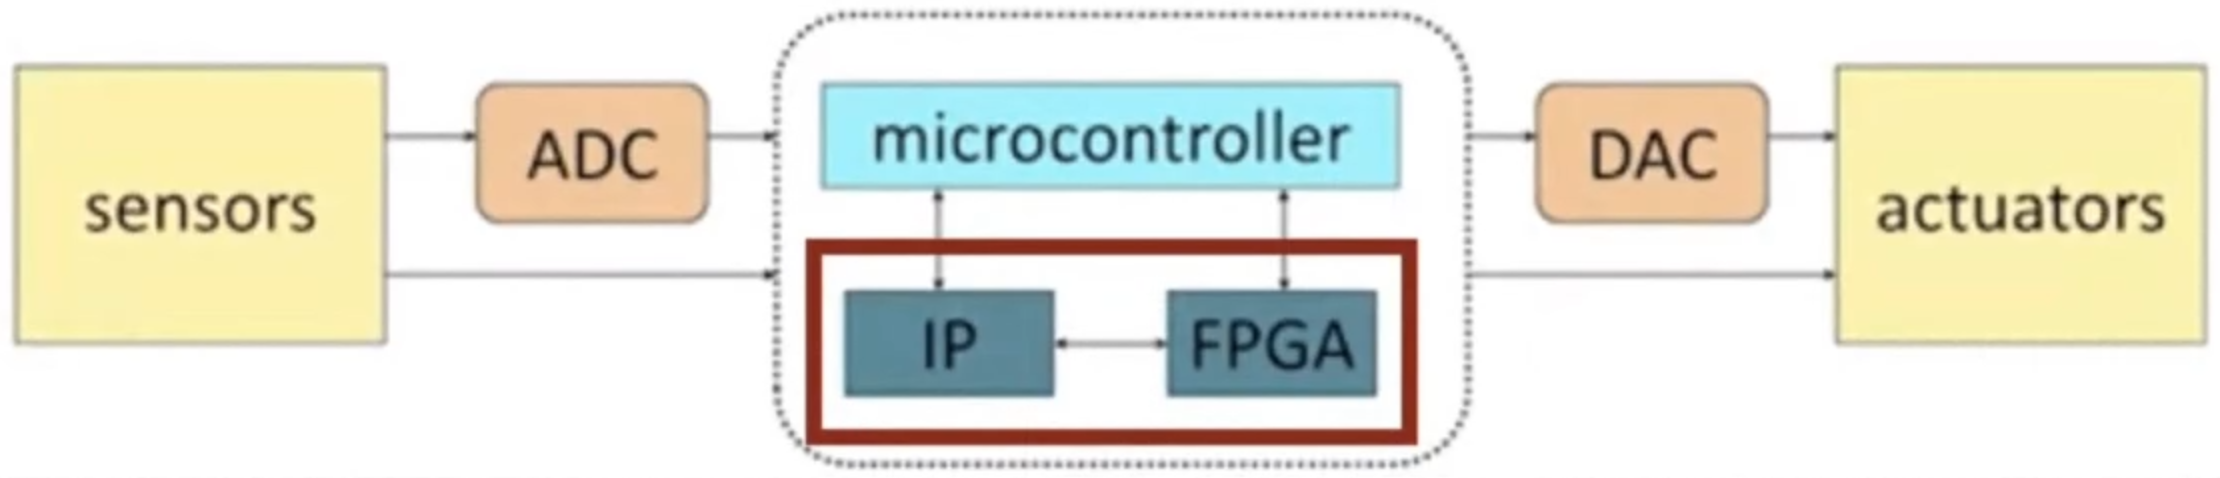
\includegraphics[scale=.35]{2021-03-19 16_58_28-DSO Elementos Sistema embebido.mkv.png}}
\end{figure}

\begin{description}
	\item[Microcontrolador] Es el componente que ejecuta un programa en un sistema integrado, y se encuentra en la zona central, se encarga de realizar el procesamiento. Recibe los datos de los sensores, procesa y envía señal a los actuadores.
	
	Consta de CPU, RAM, ROM, puertos E/S y temporizadores.
	
	Mas lento que un microprocesador, menos memoria y menos funciones.
	
	Requiere ser programado, se debe escribir el código del programa que va a realizar. El código se escribe en el host, un ordenador de sobremesa o laptop, y después se transfiere el programa del host al microcontrolador.
	\item[Cajas negras] Realizan parte del trabajo del microprocesador para reducir la carga, algunas tareas específicas. Algunos ejemplos son:
	\begin{description}
		\item[IP Core] Circuito integrado que desempeña una función que interactúa con el microcontrolador, y son baratos en un volumen alto. Muy útiles para tareas comunes como controlador de network (Ethernet, CAN)  o de audio/video (Audio Códec, Controlador VGA). Necesita interactuar con el microprocesador y se siguen unos protocolos de comunicación. 

		\item[FPGA - Field Programmable Gate Array] Matriz de puertas lógicas programable en campo, es un chip con una red de puertas de memoria RAM que se pueden configurar (establecer las conexiones entre chips o puertas), para realizar una serie de tareas, como puede ser filtrar una señal o comprimir video. Es más rápido que software, pero más lento que ASIC. 

		\item[DSP] Procesadores y compresores de señales digitales, tanto de audio como de video. Son más económicos que los procesadores, pero tiene capacidades más limitadas.

	\end{description}
	\item[Conversores] Analógico-Digital sale de sensor, izquierda y el Digital-Analógico va al actuador, derecha. Los analógico a digital son muy comunes, porque los sensores son analógicos y el microcontrolador es digital.
	\item[Sensores y actuadores] Toma medidas del medio que rodea al dispositivo y puede alterar el entorno. Sensores a la izquierda y actuadores a la derecha.
\end{description}

\section{Ejemplos de Sistemas embebidos que usamos}
\subsection{Arduino}

\begin{figure}[H]
	\ffigbox[\FBwidth]
	{\caption{Estructura Arduino}}
	{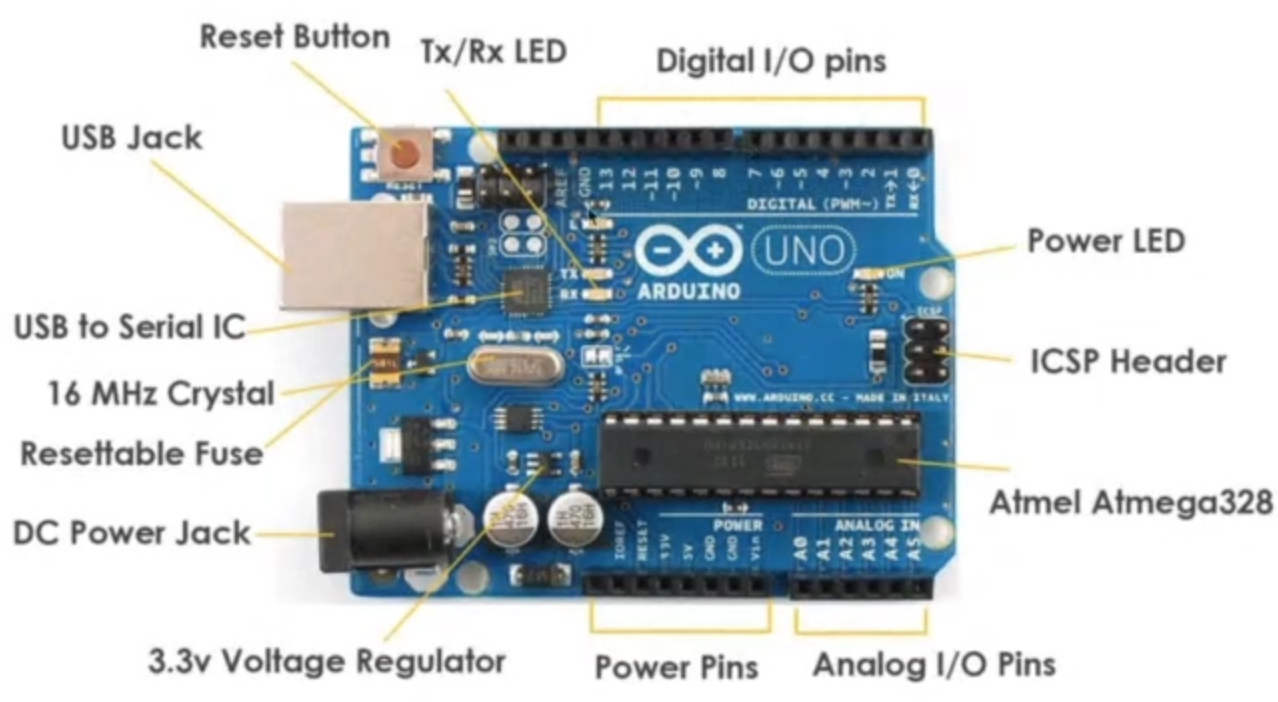
\includegraphics[scale=.5]{2021-03-19 17_31_12-DSO Elementos Sistema embebido.mkv.png}}
\end{figure}


Es una plataforma de código abierto sed para construir proyecto de electrónica.	Consta de una placa de circuito programable física (microcontrolador) y una pieza de software, o IDE (entorno de desarrollo) que se ejecuta en una computadora portátil o computadora personal utilizada para escribir y cargar código de computadora en la física. Tiene pines analógicos y digitales.
	
No necesita una pieza software separada para cargar un nuevo codigo en la placa.
	
Utiliza una versión simplificada de C++, lo que lo hace más fácil de aprender.
	
\textbf{Razones por la que se usa:} Es de código abierto, económico, multiplataforma, prototipos rápidos, entorno programable más simple y claro. Algunas también cuentan con conexión a Internet incorporada o la posibilidad de conectividad externa.
	
\textbf{Razones para no utilizarlos:} Poca memoria para datos y RAM, procesamiento, arquitectura basada en 8 bits, caro cuando se necesita a gran escala, mala calidad/precio, las empresas no les gusta que sea open source, no está aliado con proveedores y no da garantías.

\subsection{Raspberry Pi}

\begin{figure}[H]
	\ffigbox[\FBwidth]
	{\caption{Estructura Raspberry Pi}}
	{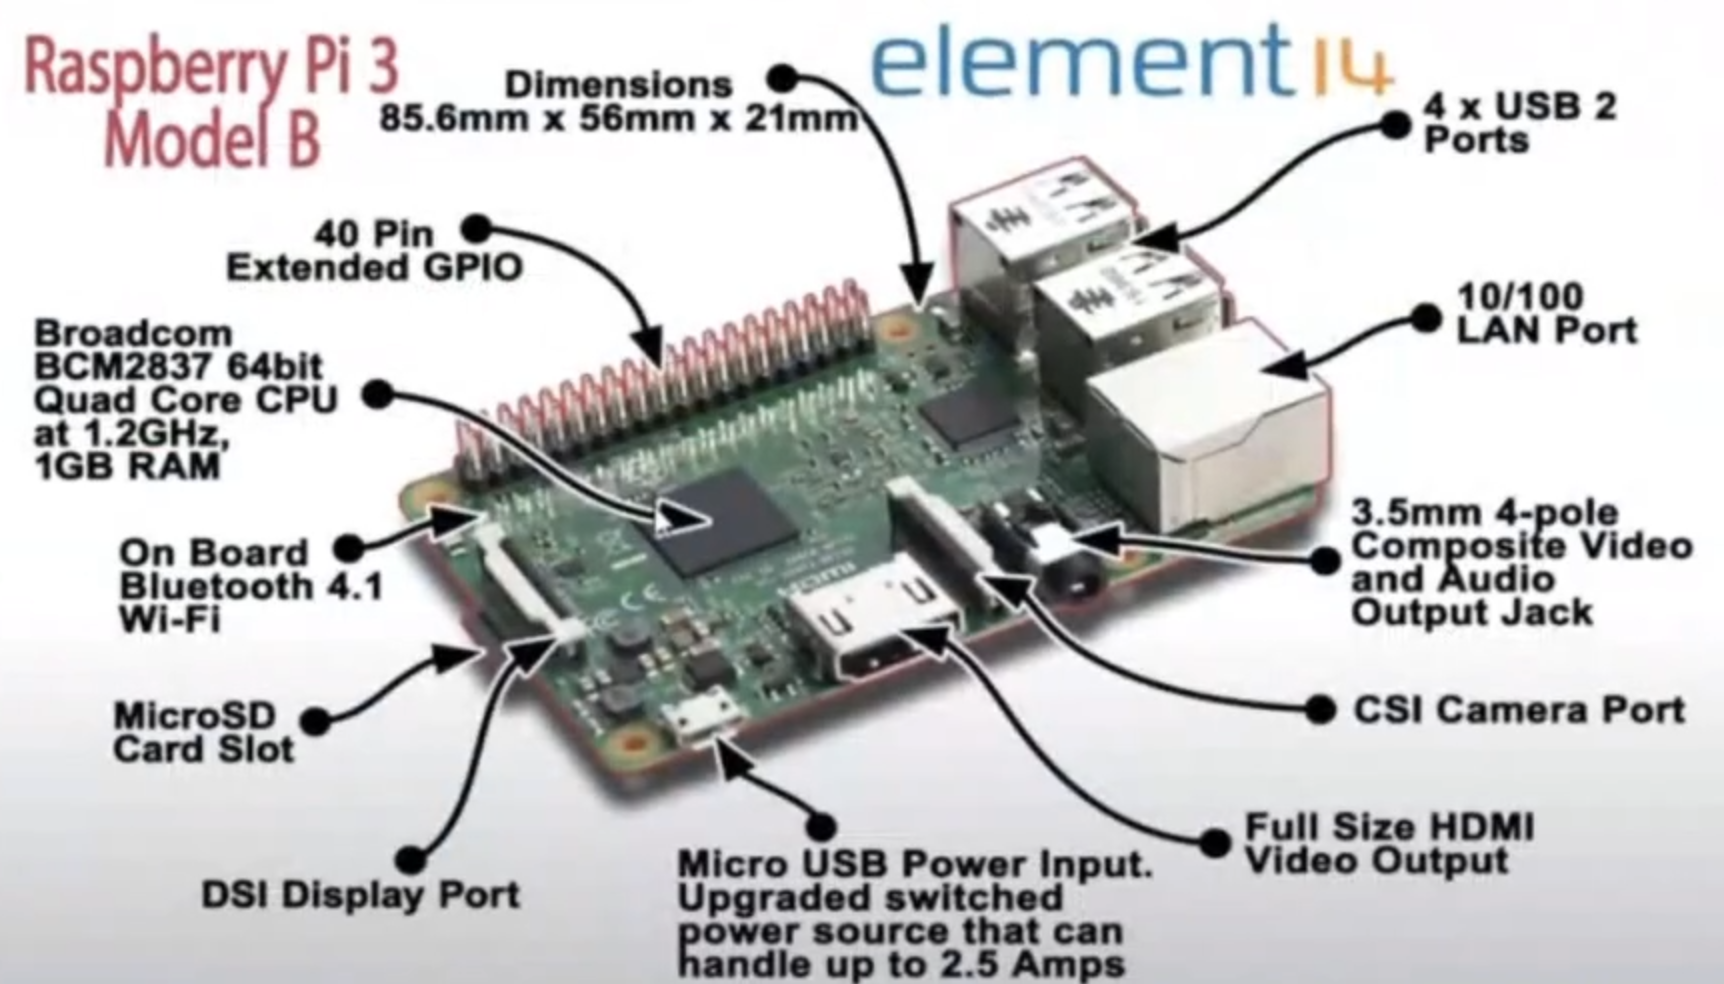
\includegraphics[scale=.4]{2021-03-19 17_48_46-DSO Elementos Sistema embebido.mkv.png}}
\end{figure}

Es una computadora de bajo costo del tamaño de una tarjeta de crédito que se conecta a un monitor de computadora o televisor y utiliza un teclado y un mouse estándar.

La Raspberry PI tiene una conexión GPIO de 40 pines, lo que facilita la conexión con el mundo exterior.


	\begin{description}
		\item[GPIO] Significa entrada/salida de uso general. Estos pines son una interfaz física entre Raspberry Pi y el mundo exterior. 
		
		El Pi puede recibir información de sensores y actuadores, y controlar actuadores como LED, ejecutar motores y muchas otras cosas.
		
		Hay 40 pines y proporcionan varias funciones diferentes. 
		\begin{itemize}
			\item Los pines 27 y 28, ID SD e ID SC, son para conectar una EEPROM.
			\item Pines 8 y 10, GPIO 14 y 15, son para comunicación UART puerto serie que transmite poca información (baja frecuencia), como USB, RFID, Bluetooth, GPS, GSM o GPRDS.
			\item GPIO 2 y 3 (clock) se usan para I2C, comunicación entre placas, como un LCD, otras placas base (Raspberry, Arduino, ...) o un reloj de tiempo real.
			\item GPIO 7, 8, 9, 10 y 11 implementan otro mecanismo de comunciación el SPI, que es la evolución del protocolo I2C, su función es comunicar full duplex, como SSD card, IP Core o Memoria Flash.
		\end{itemize}
		  
	\end{description}  
\textbf{Del cuestionario:}

\begin{itemize}

\item Cual de los siguientes NO es un beneficio de usar un sistema operativo? 

La frecuencia del reloj del microprocesador se puede aumentar significativamente.
\end{itemize}
 
\subsection{Raspberry Pi vs. Arduino}
AMPLIAR CON LAS DIAPOSITIVAS

\subsection{¿Es Raspberry Pi un dispositivo de IoT?}

\section{Sistemas Operativos embebidos}
Proporcionar una capa de abstraccion para le software sobre el sistema operativo.

Administrar los diversos recursos de hardware y software del sistema para garantizar que toto el sistema funciona de manera eficiente y confiable.

FOTO DE CAPAS Y PARTES

\subsection{Principales Sistemas Opertativos embebidos actuales} 
Zephyr, Micrium, RTOS, R IOT, VxWorks, ThreadX, MircroEJ, TinyOS, APACHE, ARMmbed, Contiki, Nucleus, Windows IoT, snappy, android things, Mongoose o mynewt.

\subsection{Requisitos de un Sistema Operativo Embebido}
\begin{itemize}	
	\item Requisitos de CPU 
	\item Requisito de Memoria, suelen tener poca memoria.
	\item Características limitadas
\end{itemize}

Autonomia
\begin{itemize}	
	\item Soporte a Plataformas
	\item Eficiencia energetica, como suspenderse bajo inactividad o protocolos de comunicacion de bajo consumo.
	\item Stack de Red Adaptativo
	\item Fiabilidad
\end{itemize}

Programabilidad: Gestionar procesos, threads, shockets...
\begin{itemize}
	\item API estandar 
	\item Lenguajes de Programación estandar 
\end{itemize}

\subsection{Modelo general de un sistema embebido}
FOTO

\subsubsection{Controladores de Dispositivos - Drivers}
Son las bibliotecas de software que sirven para interactuar con los distintos elementos hardware. Inicializan el hardware y admininistran el acceso al mismo mediante capas sueprioes de software.

Acciones:
 \begin{itemize}
	 \item Hardware Startup: 
	 Inicialización del hardware tras el encendido o el restablecimiento.
	 \item Hardware Shutdown: 
	 Configurando el hardware en su estado PowerOFF.
	 \item Hardware Disable: 
	 Permitir que otro software desactive el hardware sobre la marcha.
	 \item Hardware Acquire: 
	 Permitir que otro software obtenga acceso singular (bloqueo) al hardware.
	 \item Hardware Write: 
	  Permitir que otro software escriba datos en el hardware.
	 \item Hardware Install: 
	  Permitir que otro software instale nuevo hardware sobre la marcha.
	 \item Hardware Release: 
	  Permitir que otro software libere (desbloquee) hardware.
	 \item Hardware Unmapping: 
	 Permitiendo eliminar bloques de datos de dispositivos de almacenamiento de hardware.

 \end{itemize}

\subsubsection{Kernel}

\begin{description}
	\item[Process Management] 
	
	Threads: Crear hilos, controlarlos, terminarlos o sincronizarlos\dots

	Semaphores: Primitiva de sincronización.

	Priority scheduling:

	Real-time signal extension: Interrupciones y señales, para activaar notificaciones de aplicaciones asincronamente.

	Timers: Mecanismo de notificacion de cuando un ha ocurrido un evento como la escritura de un dato.

	.PCI.
	 
	\item[Memory Management]
	El proceso de 

	Process memory locking

	Memory mapped files

	Shared memory object

	Kernel vs user mode?
	
	\item[I/O System Management]  
	Los dispositiovs de E/S tambein deben compartirse entre los diversos procesos y, pro tanto, al igual que con la memoria, el acceso y la asignacion de un dispostivo de E/S deben adminsitrarse. 
\end{description}

\subsubsection{Middleware}

Cualquier software del sistema, que no es kernel del sistema operativo, controladores de  dispositivos o las aplicaciones que se van a desarrollar.

Controaldores de red.

Virtualizacion\dots

Middelware basico: Relacionado con la comunicacion entre... 



\paragraph{Gestion de multitareas y de procesos en sistemas embebidos}

No se pueden hacer multiples tareas a la vez, por lo que tenemos que tener un mecanimso que administre y planifique el orden de ejecucion de los distitnos procesos. Indicar ucando entran y salen, y el paso de datos.

La Rpi como tiene 4 nucleos se considera nanoordenador, no sistema embebido.


\paragraph{Implementación de procesos en Sistemas Operativos embebeidos}

Las tareas estan estructuradas como un jerarquia de tareas principales y secundarias, y cuando se inicia el kernetl embebido, solo existe una tarea.


\paragraph{Creacion de tareas}

La creación tipo “fork” crea una copia del espacio de memoria de la tarea principal en lo que se asigna para la tarea secundaria, lo que permite que la tarea secundaria herede varias propiedades, como el código del programa y las variables, de la tarea principal.

La creación tipo “exec” se utiliza para eliminar explícitamente del espacio de memoria de la tarea secundaria cualquier referencia al programa principal y establece el nuevo código de programa que pertenece a la tarea secundaria para que se ejecute.

La creación tipo “spawn model” crea un espacio de direcciones completamente nuevo para la tarea secundaria. La llamada al "modelo de generación" permite definir el nuevo programa y los argumentos para la tarea secundaria. 

Spawn model: No tiene espacios duplicados, no gasta tanta memoria como fork/exec.

fork/exec: Nos permite coordinar de una manera mas sencilla, pero es mas lenta por que tiene que copiar y elimar cuando hace el exec.

Scheduler: Es el que nos dice cuando y cuanto tiene va a ejectuar cada uno de los procesos, va metiendo y sacando de la CPU.


\paragraph{Factores clave del scheduling}

Reponse Time: Tiempo para que el programador haga que el contexto cambie a una tarea lista e incluye el timepo de espera de la tarea en cola lista.

Turnaround time: El tiempo qu tarda un proceso en completarse

Overhead: El tiempo y los datos necesarios para determinar que tareas se ejecutan  a continuación.

Fairness: ?Cuales son los factores\dots

XXX


Starvation:

\paragraph{Preventivo vs. No preventivo}

Preventivo - Apropiativo: Las tareas reciben el control de la CPU maestra hasta que finalizan su ejecucion, independientemente.

No Preventivo - No apropiativo: Se les puede expulsar de las CPU mientras ejecutan, se divide los procesos en rodajas.


\paragraph{Planificacion e Raspberry Pi OS}

Opera en todos los componentes.

Solo se ejecuta una tarea a la vez.

El planificador es un componente independiente.

El programador predetermiado es una cola FIFO simple.

El planificación es consciente de la energia, y pone el procesador en suspension cuando no hay ninguna tarea en la cola.





%\chapter{Recursos}
%\href{https://learning.oreilly.com/playlists/5a6c045f-e39c-465e-9e7c-60dcbb12aebb}{Lista de libros de referencia}
%\includepdf[pages=-]{docs/Referencias.pdf}



\end{document}
